\chapter{The Gimbal}
Once an object has been found and a desired control action calculated, the camera must be rotated so as to track it. This required the use of a camera gimbal which is powerful enough to rotate the payload specified by the researchers who will ultimately use the system: two GoPro Hero Session cameras, a distance sensor and the small camera used for tracking. Since no system was available which supports this payload, a new gimbal had to be designed and built.

\section{The gimbal frame}
There are already a number of gimbal systems available for purchase, and gimbal designs available for free use. However, the requirements of the gimbal narrowed down the options significantly. Gimbals typically need only keep a single small camera level, or rotate according to commands from an RC system. This project requires a gimbal which has space for two cameras spaced a few centimetres apart and can rotate according to commands from a Raspberry Pi. This necessitated the design of a new system.

While they couldn't be used without modification, the designs mentioned subsection \ref{ssec:gimbal_design_inspirations} were a good enough reference point that a new system could be created with relative ease.

Some priorities for the new gimbal design were as follows:

\begin{itemize}
\item It should be possible make the frame using equipment available at the university, such as a laser cutter or 3D printer.
\item It should be straightforward for someone to modify the design to house a new gadget.
\item In order to minimize the strain on actuators and the control system, there should a mechanism to help balance the gimbal.
\item As a result of the cameras being placed a few centimetres, there is an unbalanced torque. The effects of this should be minimized.
\end{itemize}
%
Based on these criterion, a gimbal was designed using SolidWorks, a CAD software used frequently in engineering design. A render of the final model used for this project is shown in Figure~\ref{fig:assembled_render}.

\begin{figure}[h!]
  \centering
  %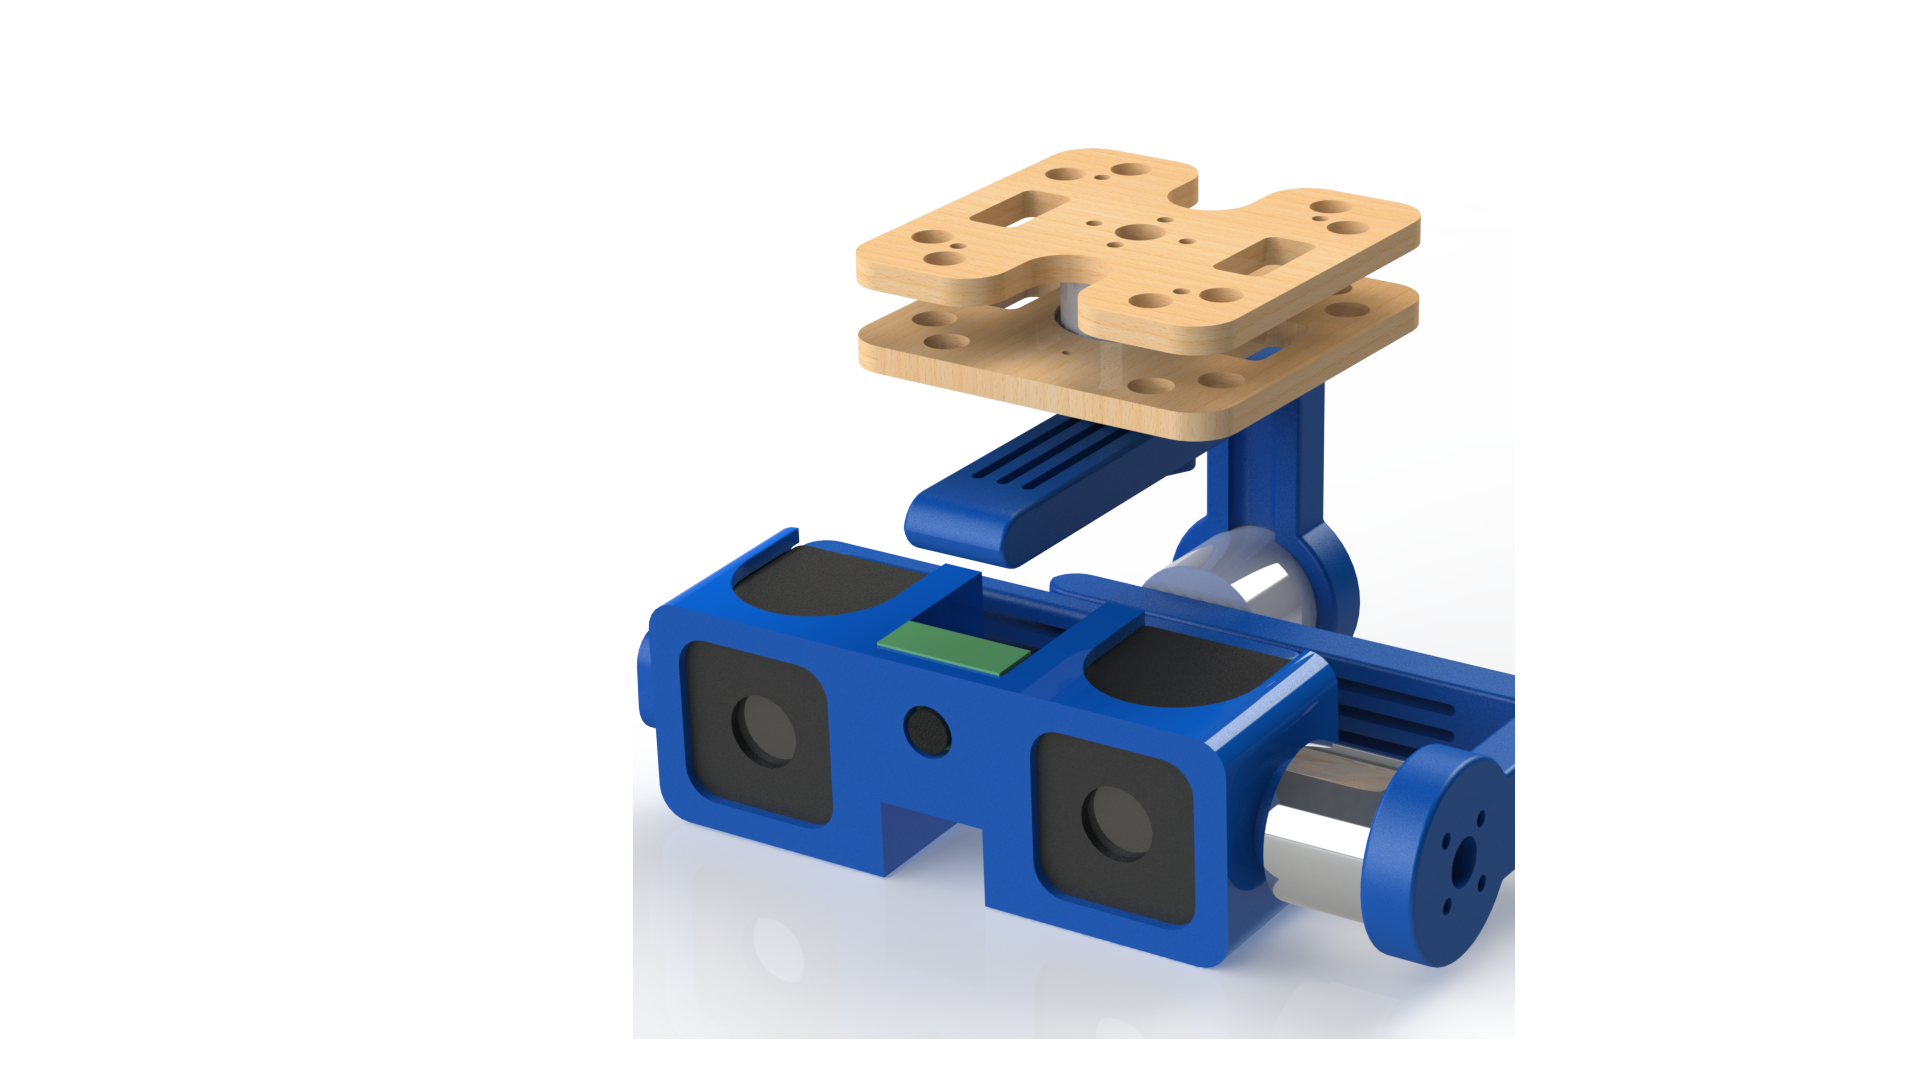
\includegraphics[width=\textwidth]{methodology/assembled_render}
  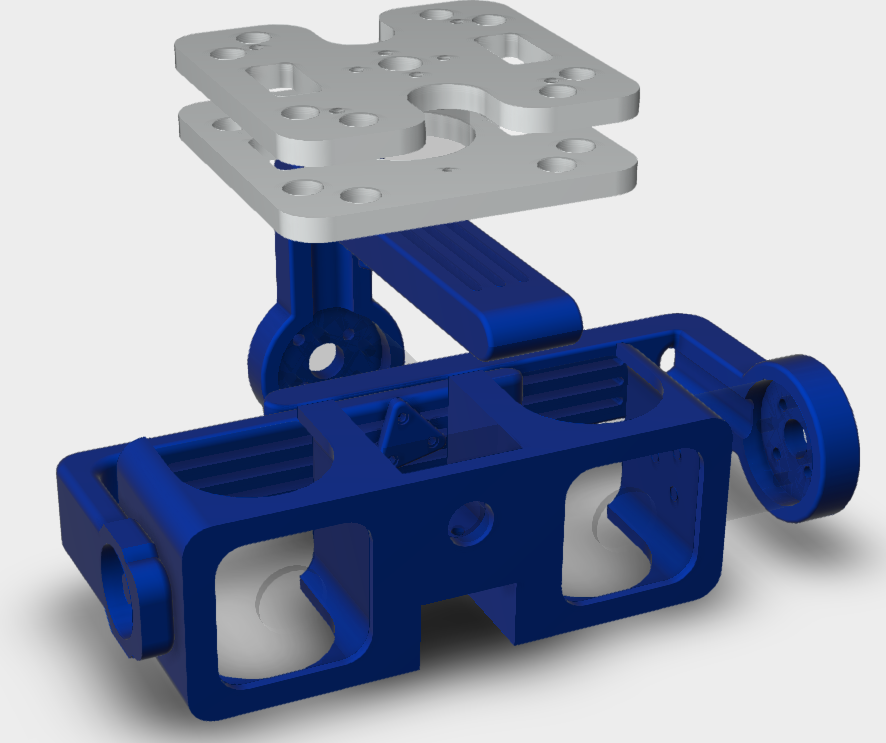
\includegraphics[width=0.7\textwidth]{methodology/assembled_render_no_cameras_motors}
  \caption{\label{fig:assembled_render} A render of the gimbal designed for this project.}
\end{figure}

The mounting panels on top were made by laser cutting hardboard, while the blue components were produced using a 3D printer.

Figure~\ref{fig:annotated_assembly_with_cams} shows the mount where the payload is placed. The GoPro's buttons can be easily reached, and there was space to place an IMU almost exactly in the center of rotation.

\begin{figure}[h!]
    \centering
    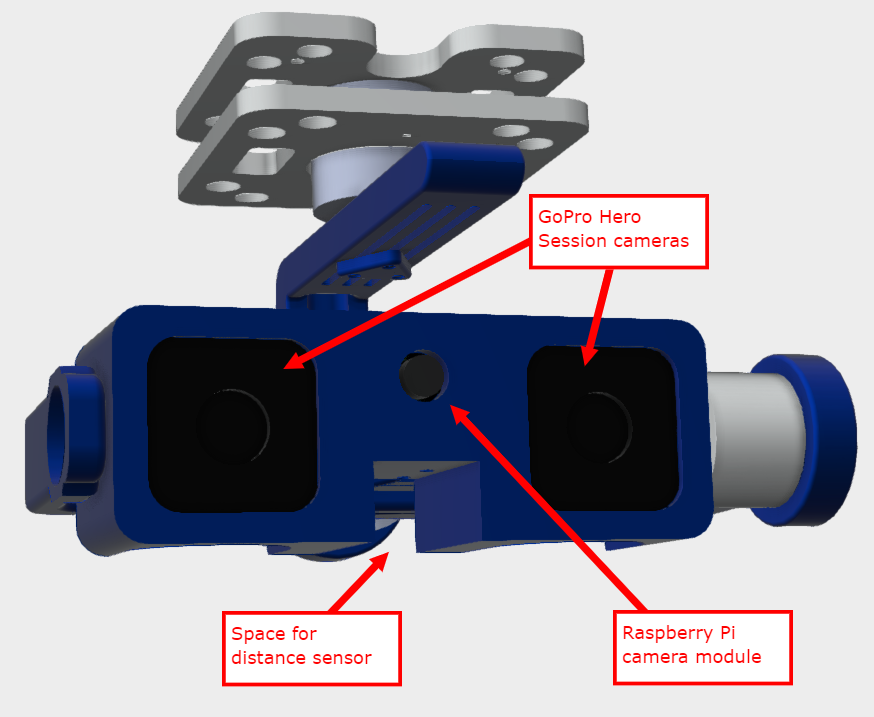
\includegraphics[width=0.7\linewidth]{methodology/annotated_assembly_with_cams}
    \caption{\label{fig:annotated_assembly_with_cams}UPDATE ME!}
\end{figure}

As can be seen in Figure~\ref{fig:annotated_assembly_no_cams}, the payload mount could be modified without needing to extend and reprint the mounting brackets. This also had the effect of making it easy to move the mass around to balance the gimbal. The addition of a support bracket mitigated the effect of a potentially large torque from the two cameras. Finally, the holes in the wooden plate on top were filled using vibration dampers.

\begin{figure}[h!]
    \centering
    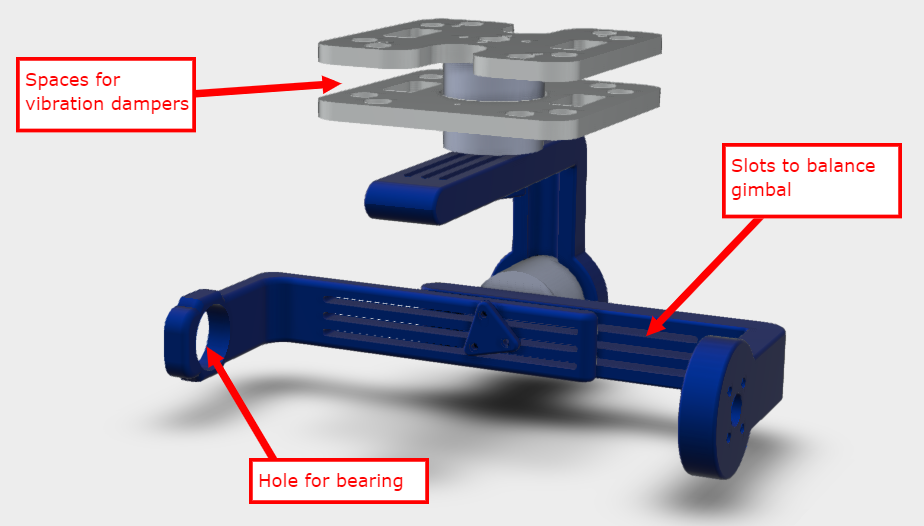
\includegraphics[width=0.7\linewidth]{methodology/annotated_assembly_no_cams}
    \caption{\label{fig:annotated_assembly_no_cams}UPDATE ME!}
\end{figure}

A final useful feature was the ability to switch between 2- and 3-axis mode by removing one of the motors and L-brackets.


\section{The gimbal controller}
Properly controlling BLDC motors to stabilize a gimbal is an entire project on its own. Luckily, there are well-designed existing products which easily fulfil the requirements needed. While research was made into the strengths and weakness of the various options available, factors such as local availability, price and time until reception of the gimbal resulted in a single actual choice: purchasing a second hand BaseCam Electronics Simple Brushless Gimbal Controller (SBGC) 32-bit controller {\color{red} (cite)} from someone who used it for drone footage.

The controller is powered off a 8-25V source and has built in power electronics, simplifying the number of components required. Up to three BLDC gimbal motors can be powered off the device.

The angular state of the gimbal is estimated using an IMU placed near the camera. The IMU contains an accelerometer and a gyroscope.

%\subsection{The Serial API}

It also has an entire serial API which allows an external computer to write commands to and read information from the gimbal. Example commands include setting motor angles and rotation rates, while those same variables can be read from the controllers built in Kalman Filter (which estimates those states).

The controllers serial API is specified in a long {\color{red} xxx} page document. The manufacturer also provides an Arduino implementation of the serial API. However, since the rest of the project was implemented in python, it was decided that the relevant communication protocol would be re-implemented in python. In addition, since a variety of users on the BaseCam forums have mentioned that they would appreciate having access to such a python module, the library will be released for free on the forums.

The serial API was made to work by looking through the specification, reading the code in the Arduino implementation and finally visualising the output of the Raspberry Pi using an oscilloscope as a last resort debugging technique.


\section{Integrating components}
Once the frame had been 3D printed, and the controller and motors purchased, the gimbal was ready for assembly and tuning.

\subsection{Gimbal motors}
Four LD-Power 2208 gimbal motors were included in the purchase of the gimbal controller. Due to the small market for gimbals, most lower-speed, higher-torque 'gimbal motors' are simply rewound high-speed quadcopter/airplane motors {\color{red} (cite)}.

The amount of torque required from a gimbal motor tends to depend more on the balance of the frame and friction in the bearings than other factors, like the rotational inertia of the objects being rotated {\color{red} (cite)}.

{\Huge \color{red} (just stop here! nothing more to see! will need to rewrite the next chapters anyway!)}

\subsubitem{Balancing the system}
talk about moving things along until the cameras would hold any angle without turning

\subsection{Tuning the controller}
selected auto-PID but this didn't work

thus, tuned them in order P $\rightarrow$ I $\rightarrow$ D $\rightarrow$ repeat.

\subsection{Testing the serial API}



